\documentclass[../main.tex]{subfiles}

\begin{document}
\chapter{Limits and Continuity}
\section{Easy Limits}
With easy limits, you can get the answer simply by plugging in the 
limiting value:
\[ \lim_{x \to 3} \frac{x^2 + x}{x + 1} = \frac{(3)^2 + (3)}{(3) + 1} = 3 \]
\section{Continuity}
\begin{defn}
    We say $f(x)$ is continuous at $x_0$ when:
    \[ \lim_{x \to x_0} f(x) = f \left( x_0 \right) \]
    \label{def:continuity}
\end{defn}
\begin{exmp}
    Consider the following \emph{piecewise} function:
    \[
        f(x) = 
        \begin{cases} 
            x + 1   & :\ x > 0\\
            -x      & :\ x \leq 0\\
        \end{cases}
    \]
    It is said to be \emph{discontinuous} 
    (see Figure \ref{fig:discontinuous-function}) at $x = 0$ 
    since we know $f(0) = 0$, but for $x > 0$:
    \[ \lim_{x \to 0} f(x) = 1 \]
    We can say $f$ is continuous from the left at $x = 0$, 
    but not the right.
\end{exmp}
\begin{defn}[Right-Hand Limit]
    \[ \lim_{x \to x_0^+} f(x) = \lim_{x \to x_0} f(x)\ :\ x > 0 \]
\end{defn}
\begin{defn}[Left-Hand Limit]
    \[ \lim_{x \to x_0^-} f(x) = \lim_{x \to x_0} f(x)\ :\ x < 0 \]
\end{defn}
\begin{figure}[h]
    \centering
    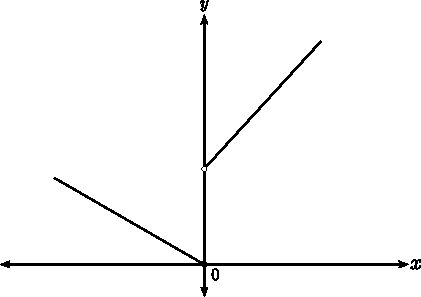
\includegraphics[width=0.5\textwidth]{discontinuous-function.pdf}
    \caption{Graph of a discontinuous function}
    \label{fig:discontinuous-function}
\end{figure}
\subsection{Discontinuities}
\begin{defn}
    A discontinuity is removable if:
    \[  
        \lim_{x \to x_0^+} f(x) =
        \lim_{x \to x_0^-} f(x) \neq
        f \left( x_0 \right)
    \]
\end{defn}
\begin{case*}
    The function $\frac{\sin(x)}{x}$ is undefined for $x = 0$. However, 
    its limit as $x \to 0$ still exists:
    \begin{figure}[h]
        \centering
        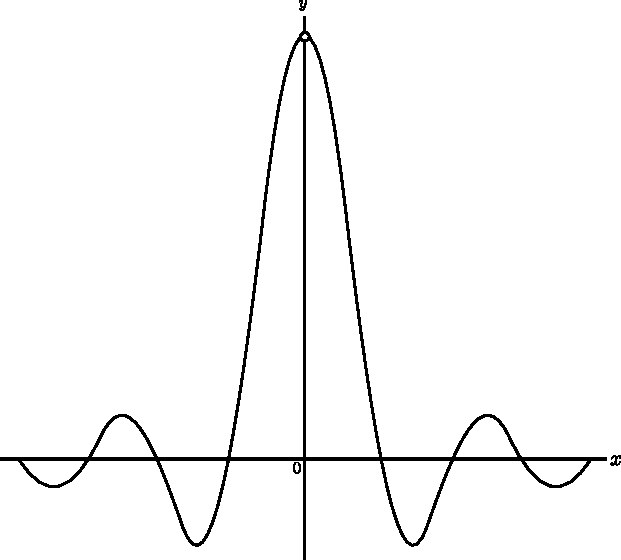
\includegraphics[width=0.5\textwidth]{removable-discontinuity.pdf}
        \caption
        {
            A removable discontinuity --- 
            the function is continuous everywhere except one point
        }
        \label{fig:removable-discontinuity}
    \end{figure}
\end{case*}
\begin{defn}
    A jump discontinuity is when 
    $\lim_{x \to x_0^+} f(x) \neq \lim_{x \to x_0^-} f(x)$ 
    even if they both exist.
\end{defn}
\begin{figure}[h]
    \centering
    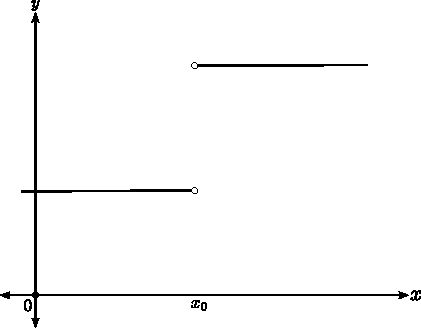
\includegraphics[width=0.5\textwidth]{jump-discontinuity.pdf}
    \caption{An example of a jump discontinuity}
    \label{fig:jump-discontinuity}
\end{figure}
\begin{defn}
    There is an infinite discontinuity when the right- and left-hand 
    limits are both infinite, but in opposite directions.
\end{defn}
\begin{case*}
    $f(x) = \frac{1}{x}$ has an infinite discontinuity
    (\emph{singularity}) at $x = 0$:
    \[
        \lim_{x \to x_0^+} \frac{1}{x} = -\infty \quad , \quad
        \lim_{x \to x_0^+} \frac{1}{x} = \infty
    \]
\end{case*}
\begin{figure}[h]
    \centering
    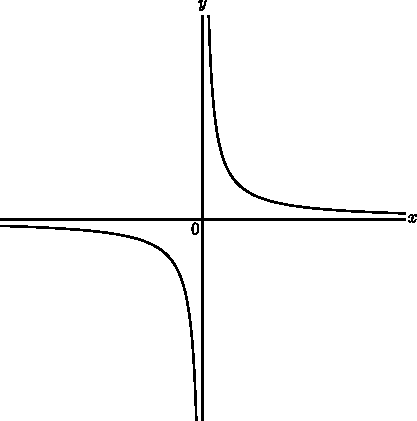
\includegraphics[width=0.5\textwidth]{infinite-discontinuity.pdf}
    \caption{$f(x) = \frac{1}{x}$ is an example of an infinite discontinuity}
    \label{fig:infinite-discontinuity}
\end{figure}
\subsubsection{Ugly Discontinuities}
The function shown in Figure \ref{fig:ugly-discontinuity} doesn't even go 
to $\pm \infty$ --- it doesn't make sense to say it "goes to" anything. 
For something like this, we say the limit does not exist (\textsc{dne}).
\begin{figure}[h]
    \centering
    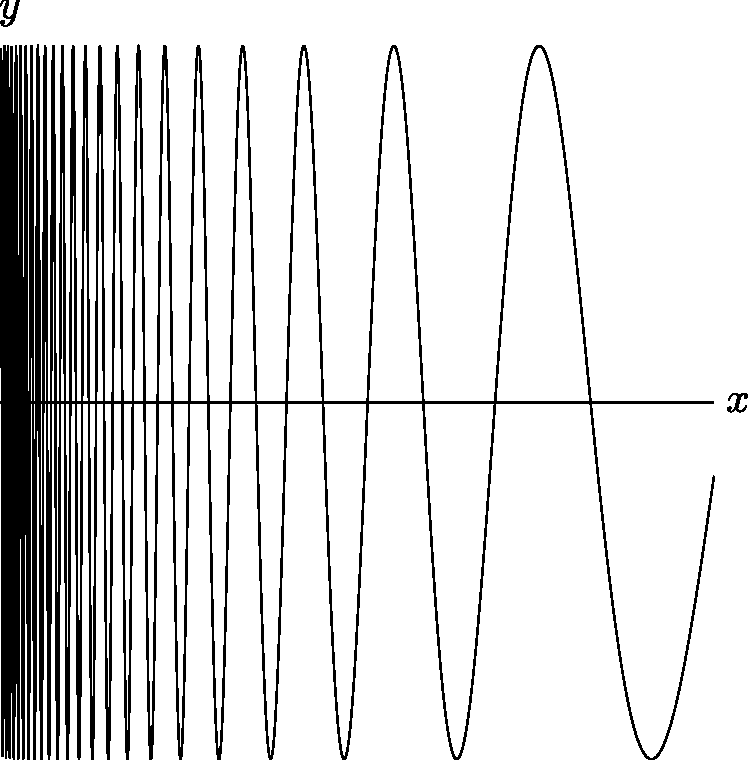
\includegraphics[width=0.5\textwidth]{ugly-discontinuity.pdf}
    \caption
    {
        An example of an ugly discontinuity: 
        a function that oscillates a lot as it approaches the origin
    }
    \label{fig:ugly-discontinuity}
\end{figure}
\section*{}
\begin{thm}
    If $f$ is differentiable at $x_0$, then $f$ is continuous 
    at $x_0$
\end{thm}
\begin{proof}
    From Definition \ref{def:continuity}, we need to show:
    \begin{align*}
        &\lim_{x \to x_0} f(x) = f \left( x_0 \right)\\
        \Rightarrow &\lim_{x \to x_0} f(x) - f \left( x_0 \right) = 0
    \end{align*}
    The \textsc{lhs} can be rewritten as:
    \begin{align*}
        \lim_{x \to x_0} f(x) - f \left( x_0 \right)
        &=  \lim_{x \to x_0} f(x) - f \left( x_0 \right)
            \cdot \frac{x - x_0}{x - x_0} \quad \because \quad
            \frac{x - x_0}{x - x_0} = 1\\
        &=  \lim_{x \to x_0} \frac{f(x) - f \left( x_0 \right)}{x - x_0}
            \cdot \left( x - x_0 \right)\\
        &=  \lim_{x \to x_0} \frac{f(x) - f \left( x_0 \right)}{x - x_0}
            \cdot \lim_{x \to x_0} \left( x - x_0 \right)
    \end{align*}
    If $f$ is differentiable, we can use Equation \ref{eqn:derivative} 
    and rearrange to get:
    \begin{align*}
        \lim_{x \to x_0} f(x) - f \left( x_0 \right)
        &=  \lim_{x \to x_0} \left( x - x_0 \right)
            \cdot f' \left( x_0 \right)\\
        &=  \left( x_0 - x_0 \right) \cdot f' \left( x_0 \right)\\
        &=  0 \cdot f' \left( x_0 \right)\\
        &=  0
    \end{align*}
\end{proof}
\begin{note}
    You can never divide by zero! The first step was to multiply by 
    $\frac{x - x_0}{x - x_0}$. It looks as if this is illegal because 
    we are multiplying by $\frac{0}{0}$ when $x = x_0$. But, when computing 
    the limit as $x \to x_0$, we always assume $x \neq x_0$. In other words, 
    $x - x_0 \neq 0$. Therefore, the proof is valid.
\end{note}
\end{document}